\documentclass[conference]{IEEEtran}
\IEEEoverridecommandlockouts
% The preceding line is only needed to identify funding in the first footnote. If that is unneeded, please comment it out.
\usepackage{cite}
\usepackage{amsmath,amssymb,amsfonts}
\usepackage{algorithmic}
\usepackage{graphicx}
\usepackage{textcomp}
\usepackage{xcolor}
\def\BibTeX{{\rm B\kern-.05em{\sc i\kern-.025em b}\kern-.08em
		T\kern-.1667em\lower.7ex\hbox{E}\kern-.125emX}}
\begin{document}
	
	\title{Arduino Uno Based Smart Bike Parking Zone\\
		

	}
	
	\author{\IEEEauthorblockN{Istyaque Ahammed \\ Student Id: 200240} 
		\IEEEauthorblockA{\textit{Computer Science and Engineering} \\
			\textit{Khulna University}\\
			Khulna, Bangladesh \\
			istyaque2040@cseku.ac.bd}
		\and
		\IEEEauthorblockN{Sumaiah Binta Musa \\ Student Id: 190205} 
		\IEEEauthorblockA{\textit{Computer Science and Engineering} \\
			\textit{Khulna University}\\
			Khulna, Bangladesh \\
			sumaiah1905@cseku.ac.bd}
	}
	
	\maketitle
	
	\begin{abstract}
		Bike parking in busy areas can be a challenge due to limited parking spots and the difficulties in detecting the presence of bikes. This study proposes a smart bike parking zone using Arduino Uno, a micro-controller based system that aims to improve the efficiency and convenience of bike parking. The system utilizes ultrasonic sensors to detect the presence of bikes in parking spots and provide real-time information on parking availability. The system also includes a user interface that allows bike riders to locate available parking spots and an interface for parking administrators to manage the parking spots remotely. The results of this study show that the smart bike parking zone using Arduino Uno is an effective solution for managing bike parking in busy areas. The system provides accurate and real-time information on parking availability and has the potential to reduce the time and effort required for bike riders to find a parking spot. The findings of this study can provide valuable insights for future improvements in smart bike parking systems.
	\end{abstract}
	
	\begin{IEEEkeywords}
		Arduino Uno, bike parking, infrared sensors, smart parking zone, real-time information, user interface, parking availability, data analysis, IoT technologies.
	\end{IEEEkeywords}
	
	\section{Introduction}
	The Arduino Uno based smart bike parking zone is a project that aims to create a more efficient and convenient system for parking bikes. The project utilizes the Arduino Uno micro-controller to control the movement of bikes in and out of the parking lot, as well as to monitor the availability of parking spaces. 
	
	\section{Related Work}
	In recent years, there has been a growing need for efficient and smart parking solutions, especially in densely populated cities. The issue of finding a parking spot is a major concern for bike riders and can often lead to traffic congestion, parking violations, and even accidents. To address this issue, several studies have been conducted to develop smart parking systems that can efficiently manage the parking spaces.
	
	One of the most common approaches for smart parking systems is the use of sensor-based technologies. In this approach, sensors are placed in the parking zones to detect the presence of vehicles and transmit the data to a central control system. For example,in [1], an IoT-based smart parking system was proposed that used ultrasonic sensors to detect the presence of vehicles and RFID technology to track the parking spots. Similarly, in [2], a smart parking system was developed using infrared sensors and a GSM module to send real-time parking information to users.
	
	Another approach for smart parking systems is the use of computer vision techniques. In this approach, cameras are installed in the parking zones to detect the presence of vehicles and analyze the parking space utilization. For example, in [3], a computer vision-based parking management system was proposed that used a deep learning algorithm to classify the parking spots and detect vehicles in real-time.
	
	While these studies have made significant contributions to the development of smart parking systems, they often require expensive hardware and technical expertise to implement. In this study, we aim to develop a smart bike parking zone using an Arduino Uno micro-controller and a set of simple sensors. Our approach is designed to be cost-effective and easy to implement, making it accessible for a wide range of users.
	
	In conclusion, the development of smart bike parking zones is an important step towards improving the efficiency of parking and reducing the challenges faced by bike riders. Our proposed solution is based on the use of a simple and affordable micro-controller and sensor setup, making it a cost-effective and accessible solution for a wide range of users.
	
	\section{MATERIALS AND METHODS}
	

	\subsection{Hardware Components:}
		 We will use these hardware items in this project, which is given below.

	\begin{itemize}
	\item Arduino Uno micro-controller
	\item Ultrasonic sensors
	\item LED lights
	\item Power supply
	\end{itemize}
	
	\subsection{Software Components:} 
		We will use these software items in this project, which is given below.
	
	\begin{itemize}
		\item Arduino IDE
		\item C programming language
		\item Serial communication protocols
	\end{itemize}
The ultrasonic sensors are used to detect the presence of motorcycles in the parking spots and provide the information to the Arduino Uno microcontroller. The LED lights are used to indicate the availability of parking spots, with green lights indicating available spots and red lights indicating occupied spots.
\begin{figure}[htbp]
	\centerline{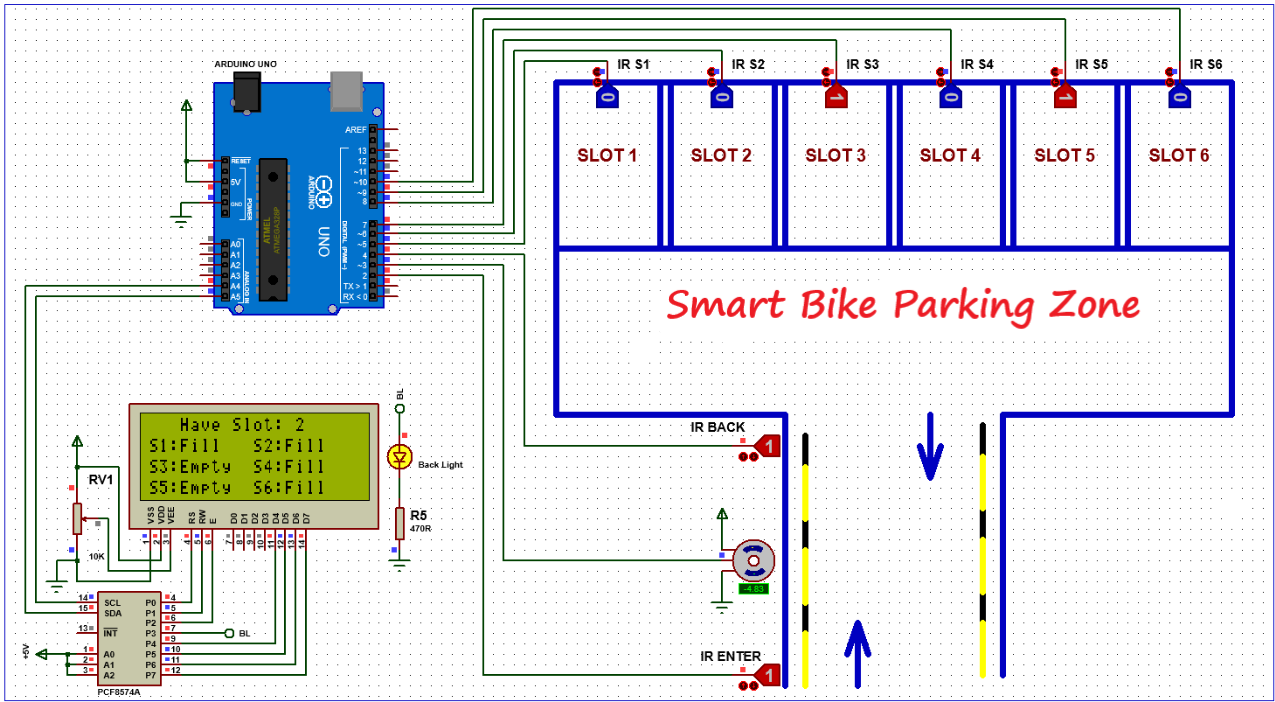
\includegraphics[scale=0.25]{Proteus Simulation.png}}
	\caption{Proteus Simulation}
	\label{fig}
\end{figure}

The Arduino Uno microcontroller is programmed using the Arduino IDE and C programming language to read the sensor data and control the LED lights. The microcontroller communicates with the user interface through serial communication protocols.

The user interface is developed using a web-based platform that allows motorcycle riders to locate available parking spots and parking administrators to manage the parking spots remotely.
	\subsection{System Architecture:}
	The smart motorcycle parking zone using Arduino Uno system consists of two primary components: the hardware and software components. The hardware components include the ultrasonic sensors, LED lights, breadboard, and Arduino Uno microcontroller. The software components consist of the Arduino IDE, C programming language.
	
	\subsection {Working Procedure:}
		A smart bike parking system using Arduino Uno can be implemented using the following working procedure.
	\begin{itemize}
		\item Set up the hardware: 
		I will need an Arduino Uno board, an ultrasonic sensor, a motorcycle driver, a DC motor, and a battery. Connect the ultrasonic sensor and motorcycle driver to the Arduino Uno board as per the instructions provided in the datasheet.
		\item Write the code:
		Write the Arduino code to control the motor driver based on the input received from the ultrasonic sensor. The code should detect the distance between the motorcycle and the parking slot and control the motor to move the bike into the parking slot.
		\item Calibrate the ultrasonic sensor: 
		Calibrate the ultrasonic sensor to ensure that it provides accurate distance measurements. Place the ultrasonic sensor at a fixed distance from a wall and use the readings to determine the scaling factor for the sensor.
		\item Test the system: 
		Test the system to ensure that it works as expected. Place a motorcycle in front of the parking slot and check if the system detects the motorcycle and moves it into the slot automatically.
		\item  Add a user interface: 
		To make the system more user-friendly, i can add a user interface such as an LCD screen or LEDs to indicate the parking slot's availability
		
		
		
		Overall, the working procedure for a smart bike parking system using Arduino Uno involves setting up the hardware, writing the code, calibrating the ultrasonic sensor, testing the system, and adding a user interface. With this system in place, cyclists can park their bikes easily and safely without worrying about theft or damage
	\end{itemize}	
		
	
	\subsection{Data Analysis:}
Data analysis is performed on the parking usage data collected from the system to provide insights into the parking behavior of motorcycle riders. The data is analyzed using statistical methods to identify patterns and trends in parking usage, which can be used to inform future improvements in the system.
	\subsection{Experimental Setup:}
	The experimental setup for the smart motorcycle parking zone using Arduino Uno system consists of a parking zone with ultrasonic sensors installed in each parking spot, an Arduino Uno microcontroller, and LED lights to indicate parking availability. The system is tested using a group of volunteers to simulate real-world usage scenarios, and data is collected on parking behavior and system performance.
	
	
	
	

	
\begin{thebibliography}{00}
\bibitem{b11}J. HANZL, "Parking Information Guidance Systems and Smart Technologies Application Used in Urban Areas and Multi-storey Car Parks," Netherlands, 2020. 
\bibitem{b2} A. J. N. A. P. R. J. et al, "Highly Secure Smart Vehicle Parking System (SVPS) for," in HBRP PUBLICATION, India, 2023 
\bibitem{b3} S. M. e. a. Aijaz, "Smart Car Parking System Using Arduino UNO," in Journal of Switching Hub 7.2 , 2022. 
\bibitem{b4}	I. G. S. M. D. e. al, "Progressive Parking Smart System in Surabaya's Open Area Based on IoT," in IOP Publishing Ltd, Indonesia, 2019. 
\end{thebibliography}

\end{document}
